% called by main.tex
%
\chapter{Marco Metodológico}
\label{ch::capitulo6}

Este capítulo tiene como objetivo detallar exhaustivamente la metodología llevada a lo largo de este trabajo de investigación con el fin de entender las decisiones y los pasos tomados para cumplir con los objetivos específicos del proyecto. A su vez, la documentación descripta a continuación servirá como base detallada para que los experimentos llevados a cabo puedan ser, en caso de ser necesario, reproducibles por terceros.

\section{Elección de datos de entrenamiento}

Como parte del objetivo de mantener la correspondencia entre el experimento de \cite{navajasAggregatedKnowledge} y el llevado a cabo en este proyecto, uno de los requisitos es asegurarnos que las predicciones de los árboles de decisión sobre el conjunto de datos de entrenamiento sigan una distribución parecida a la distribución de las respuestas de los participantes del experimento llevado en TEDx. De esta forma, siguiendo la analogía entre predicciones de árboles de decisión y estimaciones de individuos, nos aseguramos que la experimentación de nuevos mecanismos de agregación en Random Forest parte de la misma base que la experimentación en humanos.

Además, otro de los requisitos de los datasets a elegir es que sean adecuados para problemas de regresión, es decir que la variable a predecir sea continua y, a su vez, que haya diversidad entre los datasets en términos de cantidad y tipos (numéricos y categóricos) de atributos y de cantidad de observaciones. Por su parte, debíamos definir si aceptaríamos conjunto de datos con información faltante (missings) o no. Para cumplir estos requisitos fue necesario seguir un cuidado procedimiento para la elección de nuestros conjuntos de datos a utilizar en la evaluación de las alternativas.

En primer lugar, nos propusimos analizar los datos recolectados de las respuestas del experimento original. Para llevar a cabo este análisis, comenzamos solicitándole a los autores de la investigación los datos recolectados. Si bien en el experimento llevado a cabo en el evento en vivo TEDx se tomó un muestra muy grande de personas (N=5800), para el análisis posterior se decidió conservar aquellos datos correspondientes a los individuos y grupos que tenían toda la información completa (m=280 grupos, n=1400 individuos). Los autores nos compartieron efectivamente los datos filtrados y procesados.

Teniendo en cuenta que los datos tenidos en cuenta en la experimentación fueron aquellos que tenían toda la información completa, tomamos la decisión que los conjuntos de datos a seleccionar para el entrenamiento de nuestros modelos también tengan toda la información completa. 

Una vez obtenido los datos, en formato .MAT, procedimos a transformarlos en datos manejables con Python, como vectores de Numpy y archivos CSV. Dado que en el experimento, durante la segunda etapa donde ocurrían las decisiones colectivas, sólo se tenían en cuenta cuatro de las ocho preguntas que respondieron individualmente los participantes, decidimos enfocarnos en analizar la distribución sólo de las preguntas debatidas. Estas son:

\begin{itemize}
    \item ¿Cuántos goles se marcaron en la Copa Mundial de la FIFA 2010?,
    \item ¿Cuántas veces aparece la palabra “alegría” en la letra de la canción “Y dale alegría a mi corazón”?,
    \item ¿Cuál es la suma de todos los números en una ruleta?,
    \item ¿Cuánto costaba un barril de petróleo en 1970 (en centavos de dólar estadounidense)?
\end{itemize}

El primer acercamiento a los datos, como suele ser de costumbre, fue a través de realizar histogramas que nos permitan tener una primera intuición sobre la distribución de las respuestas para cada una de las preguntas del experimento. A simple vista pudimos notar que las respuestas de las cuatro preguntas seguían una distribución cercana a la forma típica de la distribución \textbf{log-normal}. 

Para confirmar esta suposición, procedimos a computar funciones de densidad log-normales ajustadas según las estimaciones de sus parámetros sobre los datos. Para ello, utilizamos la librería \texttt{scipy.stats} que permite estimar en base a los datos los parámetros:

\begin{itemize}
    \item \texttt{shape}: desvío estándar $\sigma$.
    \item \texttt{loc}: parámetro de locación sobre el eje $x$
    \item \texttt{scale}: $e^{\mu}$, mediana de la distribución.
\end{itemize}

Con estos parámetros estimados, se pueden graficar las curvas de densidad para luego contrastar con las funciones de densidad observadas empíricamente en los datos de la experimentación de Navajas\footnote{Figuras en \hyperref[appendix1]{Apéndice 1}.}. Observando las figuras vimos que, para el tipo de precisión que necesitamos, la semejanza visualmente es suficiente.

Identificada la distribución de la experimentación de \cite{navajasAggregatedKnowledge}, el siguiente paso era preparar el procedimiento que seguiríamos para evaluar datasets y determinar cuáles cumplen los requisitos de distribución. Para ello, entendimos que deberíamos tener un soporte analítico dado que no sería posible evaluarlos de manera visual. Esto se debe a que, recordando la analogía entre una fila u observación de un dataset con una pregunta, habría que analizar las distribuciones de predicciones de los árboles para cada una de las instancias de validación luego de haberse entrenado. Es sencillo notar que para datasets con miles de instancias de validación, como las que apuntamos, observar la distribución para cada una de ellas de manera visual es inviable.

Como soporte analítico para comprobar si las funciones de densidad siguen la distribución esperada, decidimos utilizar test de hipótesis ya implementados. Para comprobar la distribución log-normal aprendimos que se suele utilizar el test \textbf{Kolmogorov-Smirnov} por lo que decidimos tomar la implementación de \texttt{scipy.stats} en Python y probarlos con los datos del experimento de Navajas. Observando los resultados, vimos que el p-valor era demasiado chico, muy por debajo de $0.05$ lo cuál indicaría que debemos rechazar la hipótesis nula $H_0$ (que la distribución de los datos siguen una distribución log-normal), lo cuál se contrapone con nuestra interpretación visual. 

Profundizando en la investigación de este test de hipótesis, entendimos que el mismo es demasiado exigente para el tipo de búsqueda que estábamos realizando. Por ese motivo, decidimos seguir con otra alternativa. Esta consistió en aplicar una transformación logarítmica a los datos, con el supuesto que haciendo esto, obtendríamos que los datos transformados sigan una distribución normal. Efectivamente, esto fue lo que sucedió comprobándolo de manera visual siguiendo el mismo procedimiento utilizado anteriormente con la distribución log-normal\footnote{Figuras en \hyperref[appendix2]{Apéndice 2}.}.

Además de comprobarlo gráficamente, aplicamos un test de hipótesis, en este caso el \textbf{Shapiro-Wilk}, que mide si muestras siguen una distribución normal. En este caso, si bien ocurrió lo mismo con el p-valor como con Kolmogorov-Smirnov, en este caso los valores del estadístico del test se aproximaban mucho a 1, lo que indica que la distribución se encuentra muy cercana a la distribución normal \footnote{Tabla en \hyperref[appendix3]{Apéndice 3}.}. Vemos que el promedio de este estadístico para las cuatro preguntas es $0.9809$.

Completado el análisis sobre los datos del experimento, creamos un código en Python que dado un dataset:

\begin{enumerate}
    \item Se divide entre conjunto de entrenamiento y validación.
    \item Se entrena un modelo de Random Forest tradicional con el conjunto de entrenamiento con 100 árboles de decisión.
    \item Por cada instancia de validación se toman las predicciones de los 100 árboles de decisión, se le aplican una transformación logarítmica para luego aplicarles el test de hipótesis de Shapiro-Wilk.
    \begin{enumerate}
        \item En caso de que el valor del estadístico resultante esté en el rango de un $\pm 10\%$ del promedio del estadístico sobre los datos de Navajas ($0.9809$) se toma como caso favorable.
        \item Caso contrario, se toma esa instancia como no favorable.
    \end{enumerate}
    \item Se computa el porcentaje de instancias favorables sobre la totalidad, para obtener nuestro porcentaje de aceptación de un dataset.
\end{enumerate}

Analizados unos 30 datasets de fuentes como \textit{OpenML} y \textit{Kaggle}, fuimos generando un ranking de los mismos en base al porcentaje de aceptación computado\footnote{Tabla en \hyperref[appendix4]{Apéndice 4}.}. Observando los resultados, decidimos tomar como datasets principales para la experimentación \textit{House 8L}, \textit{Wind Speed} y \textit{Carbon Footprint} dado que están entre aquellos con mayor porcentaje de aceptación de distribución. Además, entre los datasets seleccionados, hay diversidad en cantidad de instancias y cantidad de \textit{features} (columnas). En el caso de \textit{House 8L}, se predice el precio de una casa basado en características numéricas exclusivamente, mientras que en \textit{Wind Speed}, se predice la velocidad del viento a partir de variables como precipitación, temperatura y fecha. Por su parte, en \textit{Carbon Footprint}, se estima la emisión de carbono de individuos basada en sus consumos de energía e insumos, como que tipo de transporte utiliza y la cantidad de ropa nueva comprada al mes.

Una vez seleccionados los principales conjuntos de entrenamiento, procedimos a analizar con mayor profundidad su conformación\footnote{Fuente de los datasets en \hyperref[appendix5]{Apéndice 5}.} y realizar ingeniería de atributos en las columnas necesarias de cada uno de ellos:

\begin{itemize}
    \item \textit{House 8L}: Este conjunto de datos no requirió modificaciones, ya que todas sus columnas son numéricas y no identificamos la necesidad de realizar transformaciones.
    \item \textit{Wind Speed}: Este dataset contiene una columna llamada \texttt{DATE}, donde las fechas están formateadas como Año-Mes-Día. Para simplificar el análisis y reducir la cantidad de columnas generadas mediante técnicas como \textit{One-Hot Encoding} (OHE), desglosamos esta columna en tres nuevas: \texttt{Year}, \texttt{Month} y \texttt{Day}.
    \item \textit{Carbon Footprint}: Este conjunto de datos presentaba dos columnas que requerían transformaciones: \texttt{Recycling} y \texttt{Cooking\_With}. Por ejemplo, la columna \texttt{Cooking\_With} contenía listas de valores como \texttt{["Microwave", "Grill", ``Airfryer'']}. Para facilitar su análisis, creamos columnas binarias para cada elemento de las listas, resultando en nuevas columnas como \texttt{Cooking\_With\_Microwave}, \texttt{Cooking\_With\_Grill} y \texttt{Cooking\_With\_Airfryer}. Aplicamos el mismo enfoque a la columna \texttt{Recycling}.
\end{itemize}

A su vez, además de estos 3 conjuntos de entrenamiento, decidimos tomar tres conjuntos más que tenían un porcentaje de aceptación más bajo sobre la distribución. De esta forma, con los mismos podríamos evaluar también si la distribución log-normal de las predicciones iniciales de los árboles de decisión es un factor determinante para las modificaciones o no. Entre estos datasets adicionales se encuentra \textit{Abalone}, conjunto de datos utilizado en \cite{breimanRF}, \textit{Rainfall} y \textit{Flight price}.


\section{Configuración del entorno}
\label{confi-entorno}

Como mencionamos previamente en el marco teórico, utilizamos un entorno virtual para instalar todas las herramientas necesarias a lo largo del proyecto con dos objetivos principales. En primer lugar, evitar problemas de compatibilidad entre las distintas herramientas y, por otro lado, asegurarnos de que cada una de las computadoras utilizadas para el proyecto tenga exactamente la misma configuración.

Dentro del entorno, instalamos la versión editable de Scikit-Learn, descargando su versión \texttt{1.6.dev0} el día 19 de agosto del 2024, y partimos de esa versión para realizar todos nuestros cambios, asegurando que ninguna actualización nos cause problemas y que los experimentos sean bajo las mismas condiciones. Esta versión editable, además, nos permitió probar de manera muy sencilla nuestros cambios, ya que está preparada para reflejar inmediatamente cualquier cambio hecho al código de la biblioteca sin necesidad de realizar ningún tipo de re-instalación.

El paso por paso para configurar este entorno, ya sea desde una computadora Linux o Windows se puede encontrar en el \hyperref[appendix6]{Apéndice 6}.

\section{Decisiones implementativas}

Con respecto a la implementación de los experimentos, para cumplir con las buenas prácticas de la librería \textit{Scikit-Learn} y buscar mantener el código original sin modificaciones, optamos por usar herencia de clases por los motivos anteriormente descriptos en el Marco Teórico.

En primer lugar, identificamos, dentro de la totalidad de la librería, que para nuestro proceso de experimentación debíamos utilizar como base la clase \textbf{\texttt{RandomForestRegressor}} que implementa el algoritmo de Random Forest original. A partir de allí, entendimos que todas nuestras alternativas de RF iban a tener en común el proceso de agrupamiento de los árboles para la posterior “deliberación” entre los mismos.

Con ese supuesto, decidimos implementar la clase \textbf{\texttt{RandomForestGroupDebate}}, la cuál hereda de \texttt{RandomForestRegressor}. La misma agrega a la implementación original la funcionalidad de poder agrupar tanto los árboles de decisión en sí (método \texttt{group\_split()}), como las predicciones independientes de los mismos (método \texttt{group\_split\_predictions(predictions)}). Ambos métodos dividen el conjunto de árboles en subgrupos, controlados por el nuevo parámetro de los modelos: \texttt{group\_size} (tamaño de los grupos).

Una vez definida esta clase “base”, las distintas variantes del modelo que buscan simular el “debate” entre árboles heredan \texttt{RandomForestGroupDebate} para ya tener incorporada la funcionalidad de agrupamiento, sin necesidad de re-implementarla. Es así como las nuevas clases cuentan con adaptaciones o re-implementaciones de los dos métodos fundamentales, \texttt{fit} y \texttt{predict}, de acuerdo a los distintos enfoques de simulación de la deliberación. 

Además, reutilizamos la función de paralelización de predicciones de árboles de la implementación original, la cuál aporta como mecanismo para hacer más eficiente el cómputo de las predicción sobre nuevos datos. Para algunas de las implementaciones de alternativas, realizamos un ajuste sobre la misma. En lugar de acumular las predicciones en una suma, la función se modificó para almacenarlas individualmente.

\section{Modelos de simulación del debate}

En esta sección se detallan las diferentes alternativas al RF exploradas e implementadas que incorporan etapas intermedias entre las predicciones de los árboles de decisión y su agregación, buscando imitar y simular la deliberación y búsqueda de predicciones consensuadas dentro de los grupos.

\subsection{Exclusión de extremos}

En esta alternativa exploramos la idea de simular la exclusión de “opiniones extremas” dentro de un debate para así evaluar si esto mejora la predicción colectiva del grupo y crea un consenso más equilibrado y menos variable.  Esta idea surge del supuesto de que probablemente durante el debate entre personas, si hay un consenso de que algunas predicciones individuales están muy alejadas de la mayoría, aquellas más extremas serán excluidas de la predicción final. 

En primer lugar, nos pareció oportuno utilizar método de exclusión de valores atípicos (\textit{outliers}) con el \textit{Rango Intercuartil} (Interquartile Range o IQR en inglés). Este método tiene un extendido uso en el área de estadística y análisis de datos, popular  por su uso para los gráficos de boxplots.

Para ello, ideamos el modelo \textbf{\texttt{IQRRandomForestRegressor}}. El mismo, se implementa mediante una clase con el mismo nombre que sobrescribe el método \texttt{predict} de \texttt{RandomForestRegressor} para poder filtrar valores extremos en las predicciones individuales de los árboles. Para hacerlo, en primer lugar, se calcula el IQR de las predicciones individuales de los árboles en cada grupo usando el primer cuartil (Q1) y el tercer cuartil (Q3), donde:
\[
IQR = Q3 - Q1
\]

Luego, se descartan las predicciones que se encuentren fuera del rango de aceptación, definido como:
\[
[Q1 - 1.5 \cdot IQR, Q3 + 1.5 \cdot IQR]
\]

Una vez obtenidas las predicciones aceptadas, se computa la media de las predicciones que quedaron en cada grupo para así conformar la predicción del grupo. Finalmente, se promedian los resultados de todos los grupos para obtener la predicción final del modelo \texttt{IQRRandomForestRegressor}.

En segundo lugar, como otra alternativa de exclusión que permita explorar rangos definidos por el mismo usuario, ideamos el modelo \textbf{\texttt{PercentileTrimmingRandomForestRegressor}}. El mismo fue implementado con una clase que sobrescribe la función \texttt{predict} de la clase original para también filtrar las predicciones extremas de los árboles pero utilizando percentiles variables.

Para ello, cuenta con un hiperparámetro llamado \texttt{percentile}. El mismo funciona de manera tal que si, por ejemplo $percentile = 2$, entonces $p_{inf}$ (el percentil inferior) es el número que deja un $2\%$ de los datos a izquierda y $p_{sup}$ (el percentil superior) el que lo hace a derecha.

En en este algoritmo entonces, para cada grupo de predicciones, se calculan los percentiles inferior y superior ($p_{inf}$ y $p_{sup}$), definidos por el mencionado hiperparámetro y una vez calculados dichos valores, se eliminan las predicciones fuera del rango:
\[
[p_{inf}, p_{sup}]
\]

Finalmente, al igual que en IQR, se calcula el promedio de las predicciones aceptadas de cada grupo y se obtiene la predicción final promediando todos los grupos.

Es importante notar que IQR y Percentile Trimming son métodos distintos. IQR calcula límites \textbf{dinámicos} basados en la dispersión de los datos (Q1 y Q3), mientras que Percentile Trimming utiliza percentiles \textbf{fijos} definidos por el usuario. Además, Percentile Trimming siempre elimina valores extremos, mientras que IQR podría no hacerlo si todas las predicciones se encuentran dentro del rango calculado. Por estas razones, no existe un valor de percentil que coincida exactamente con los límites del IQR.

\subsection{Media ponderada por confianza}

Este enfoque busca simular un debate en el que cada participante tiene un peso proporcional al nivel de confianza en sus argumentos para conformar la predicción consensuada grupal. Es así como, aquellos árboles con un mayor nivel de confianza, determinada por su historial de predicciones correctas, influyen más en la decisión grupal.

Este concepto fue ejecutado mediante el modelo \textbf{\texttt{OOBRandomForestRegressor}}. El mismo, también implementado con una clase que hereda de \texttt{RandomForestRegressor}, sobrescribe el método \texttt{fit} para, además de construir los árboles de decisión independientes, calcular el \textit{nivel de confianza} de cada árbol.

Definimos la \textit{confianza} como la capacidad del árbol para predecir correctamente sobre aquellas muestras no seleccionadas durante el proceso de \textit{bootstrapping} y por lo tanto no utilizó para su entrenamiento. Estas observaciones del conjunto de entrenamiento son las ya mencionadas muestras \textit{Out-Of-Bag} (OOB), de aquí el nombre del modelo. Son estas observaciones las que serán evaluadas, como si fuesen el conjunto de validación, para medir la performance del árbol prediciendo mediante el error cuadrático medio (MSE). 

Esta performance, medida en MSE, será la base para la conformación del \textit{nivel de confianza} de cada árbol. Para ello, se le asigna a cada árbol un peso inverso de forma que los árboles con menor MSE tengan mayor peso. Así, quedan conformados como: 
\[
w_i = \frac{1}{MSE} \,\, \forall \,\, \mathrm{tree_i} \in \mathrm{Trees}.
\]

Finalmente, dentro de cada grupo, se normalizan dichos pesos de manera lineal para conformar la “confianza” como:
\[
c_i = \frac{w_i}{\sum_{j=0}^{s} w_j}\,, \; \text{donde} \,\, \mathrm{s = group\_size}.
\]

Por su parte, en el método \texttt{predict}, se buscan las predicciones de los árboles en cada grupo y con los índices de confianza calculados en \texttt{fit} se computa la media ponderada de las predicciones de los árboles en cada grupo como:
\[
\hat{Y} = \sum_{i=0}^{s} \, \hat{y}_i \cdot c_i
\]

Finalmente, como en todos los modelos, aplicamos la agregación simple de la media entre todas las predicciones de cada grupo.

Habiendo implementado esta alternativa, surgió de manera natural preguntarnos qué sucedería si combinamos esta idea de niveles de confianza de los árboles junto con la idea de exclusión de extremos para así, modelar una deliberación más compleja. De esta forma, surgió la ideación del modelo \textbf{\texttt{OOBPlusIQRRandomForestRegressor}} que combina las simulaciones implementadas en \texttt{IQRRandomForestRegressor} y \texttt{OOBRandomForestRegressor}.

En este modelo, se computan durante entrenamiento los pesos inversos $w_i$ de cada árbol con el MSE calculado sobre las instancias OOB. Pero, a diferencia de \texttt{OOBRandomForestRegressor}, los índices de confianza deberán determinarse en este caso durante predicción dado que se deben excluir de la normalización aquellos pesos de los árboles cuyas predicciones quedaron fuera del rango de IQR.

Entonces, el método \texttt{predict} se encargará en primer lugar de obtener y agrupar las predicciones iniciales de los árboles. Luego, al igual que en \texttt{IQRRandomForestRegressor} se descartan las predicciones consideras \textit{outliers} y, finalmente, se computan los índices de confianza sólo sobre aquellos árboles cuyas predicciones no fueron excluidas. Es así como, en este caso la predicción final del grupo estará dada por:
\[
\hat{Y} = \sum_{i=0}^{s} \hat{y}_i \cdot c_i \; \forall \; \hat{y}_i \in \mathrm{[Q1 - 1.5 \cdot IQR, Q3 + 1.5 \cdot IQR]}
\]

\subsection{Combinación de árboles}

La idea de combinar los árboles pertenecientes a cada grupo busca simular cómo, en algunos casos, la deliberación y búsqueda de respuestas consensuadas no pasa por simplemente combinar las predicciones individuales, sino que por el contrario, se buscan compartir los argumentos e ideas para conformar un nuevo razonamiento grupal.

Análogamente a pensar en partes pequeñas del razonamiento de los individuos, se pueden pensar a los cortes o divisiones de cada nivel de partición de los árboles de decisión como la unidad mínima en la que se puede dividir el “razonamiento” de la estructura de los árboles de decisión. A su vez, como se detalló en el marco teórico, la jerarquía de las particiones en los árboles de decisión siguen la lógica de que aquellas más cerca de la raíz del árbol son aquellas que más información aportan para la toma de decisión para la predicción final.

Con estas ideas en mente, surgió el modelo \textbf{\texttt{FirstSplitCombinerRandomForestRegressor}}, el cuál durante entrenamiento, una vez construidos los árboles iniciales independientes, se los agrupa y combina generando así un único árbol por grupo. Para conformar este árbol único, basándonos en la premisa de que los primeros cortes de cada árbol son los que contienen mayor información, se toman y almacenan cuáles fueron las columnas (\textit{features}) y valores de corte (\textit{thresholds}) de cada nodo raíz de los árboles del grupo. Con esta información es que se construirá un nuevo árbol representativo de “primeros cortes”, con el objetivo de aprovechar al máximo la información más significativa.

Para implementar esta alternativa, no solo requirió modificar los métodos \texttt{fit} y \texttt{predict}, sino también implementar un nuevo mecanismo de construcción de los árboles. Dado que la implementación original de construcción de árboles se encuentra en la sección de la librería implementada en Cython, decidimos también hacerlo en ese lenguaje y heredar la clase encargada originalmente de la construcción llamada \texttt{DepthFirstTreeBuilder}. En la nueva clase heredada, re-implementamos el método \texttt{build} para que ahora a partir de las \textit{features} y \textit{thresholds} de los primeros cortes de los árboles se construya un nuevo árbol.

Esta construcción está dada por tomar cada nodo raíz de los árboles iniciales y concatenarlos a lo largo de los niveles del nuevo árbol, así combinando las decisiones iniciales de cada árbol para conformar nuevos caminos de decisión. Es decir, el nodo raíz del nuevo árbol será, por ejemplo, el nodo raíz del primer árbol del grupo y sus nodos “hijos”, tanto a izquierda como a derecha, serán el nodo raíz del segundo árbol del grupo, y así sucesivamente. En la \hyperref[figure2]{Figura 2}, se puede observar un ejemplo ilustrativo de cómo quedará conformado un árbol combinado a partir de tres árboles iniciales. Se puede notar, como la profundidad de los nuevos árboles combinados estarán dados por el tamaño de los grupos conformados.

\begin{figure}[h]
\centering
    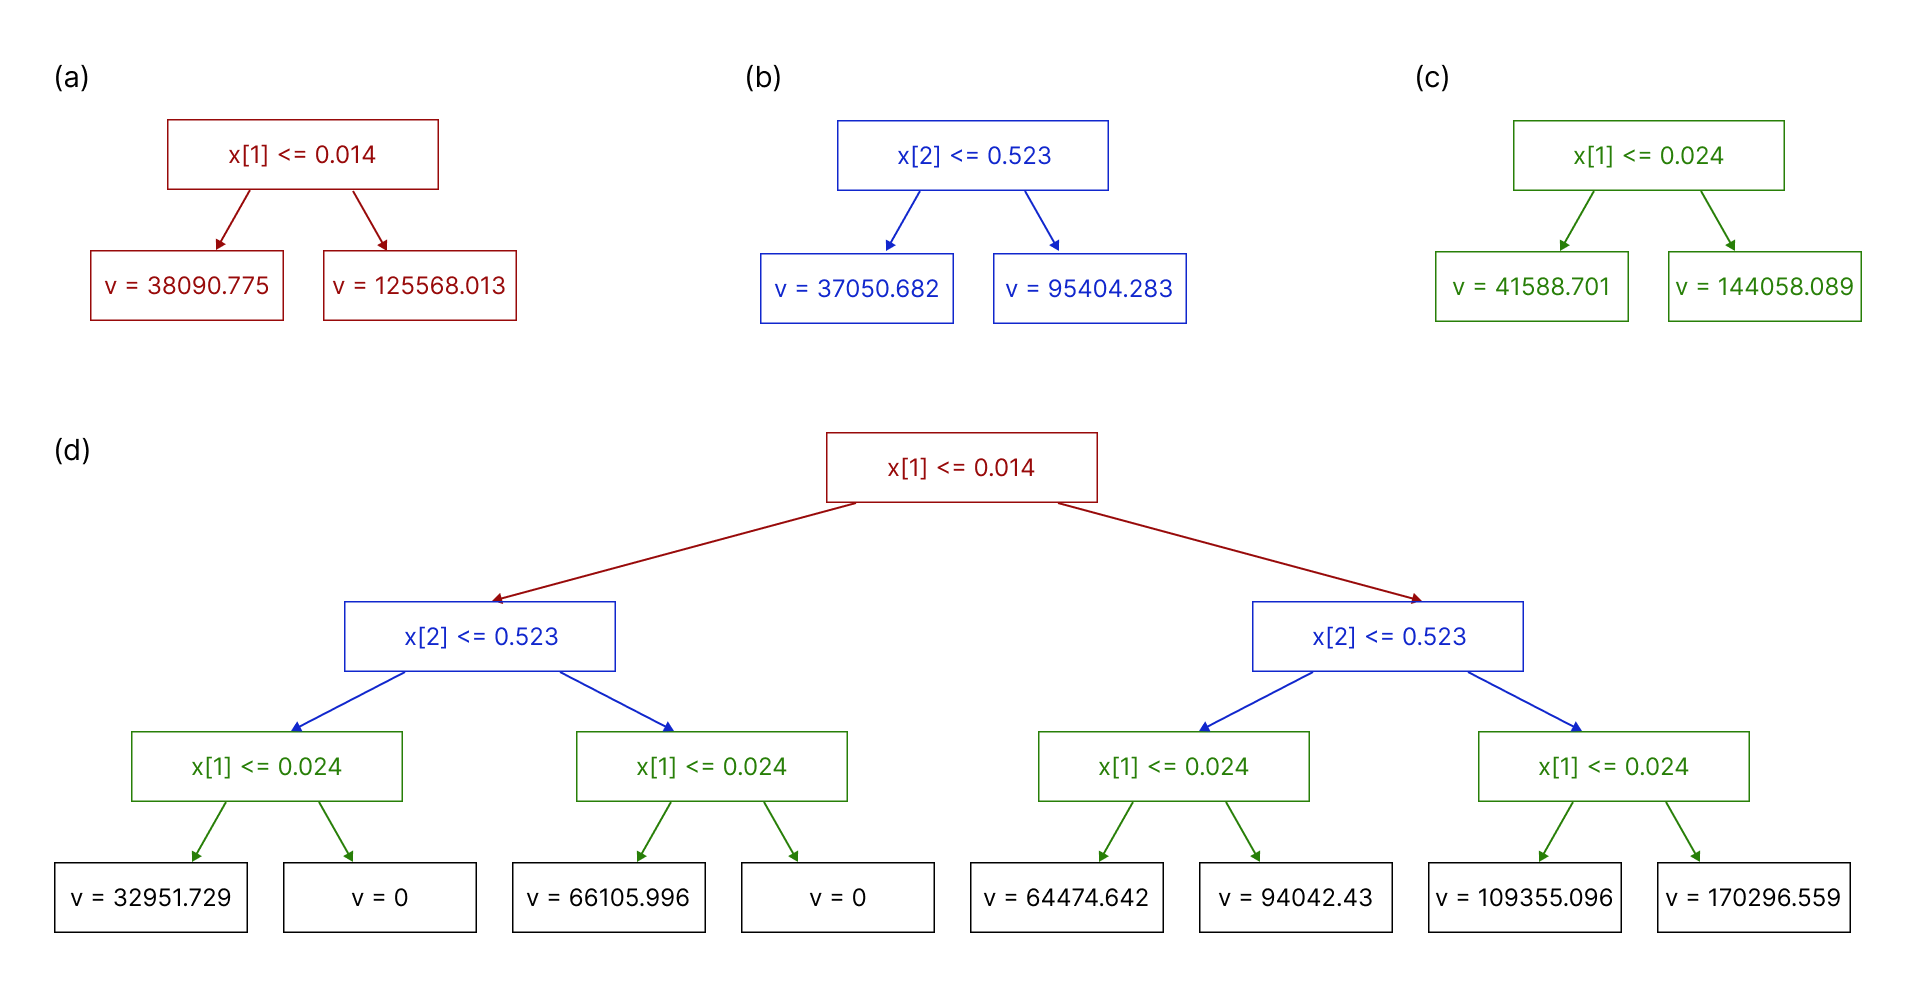
\includegraphics[width=1\textwidth]{figures/marco-metodologico/FSC.png}
\caption{Ejemplo ilustrativo de combinación de árboles dónde (a), (b) y (c) son los árboles iniciales y (d) es el combinado resultante.}
\end{figure}
\label{figure2}

Habiendo discutido el mecanismo de construcción de los nuevos árboles, entonces, el modelo \texttt{FirstSplitCombinerRandomForestRegressor} durante entrenamiento con el método \texttt{fit} se agrupan los árboles iniciales, obtiene la información relevante de los nodos raíz de cada uno de ellos y se ejecuta la construcción cada uno de los nuevos árboles de cada grupo con el nuevo constructor definido e implementado en Cython. Este constructor crea los nodos necesarios según la estructura de árboles de la librería y luego se computan los valores de las hojas según la unión de las muestras utilizadas por los árboles iniciales del grupo.

Una vez conformados los nuevos árboles en entrenamiento, al querer predecir sobre nuevas instancias se deberá llamar al método \texttt{predict} que, de forma paralela, computará la predicción de cada grupo para cada observación utilizando los árboles de primeros cortes combinados. Al igual que siempre, las predicciones de cada grupo serán promediadas para obtener la predicción final del modelo.

Este modelo tiene algunas particularidades implementativas que valen la pena resaltar. En primer lugar, dado que de los árboles de decisión iniciales sólo se toman los primeros cortes, nos pareció oportuno que al construirse, se hagan con una profundidad limitada de un sólo nivel. De esta forma se acelera mucho el proceso de cómputo del entrenamiento del modelo.

Por otro lado, cuando se realizan entrenamientos con grupos de más de 20 árboles (regulado por el hiperparámetro \texttt{group\_size}), el algoritmo sufre problemas de memoria, en particular el problema \textit{OOM Killer} (\textit{Out of Memory}), debido a la elevada cantidad de información se debe almacenar de los árboles iniciales. De todas formas, llevándolo nuevamente a la analogía, así como es muy difícil que muchas personas debatan y lleguen a un acuerdo, no nos parece que tenga sentido armar grupos de muchos árboles tampoco.

\subsection{Conocimiento compartido entre árboles}

En esta alternativa, buscamos emular cómo el intercambio de “conocimiento” entre individuos puede influir en sus decisiones. Los participantes ajustan sus argumentos tras intercambiar puntos de vista y recibir retroalimentación durante la deliberación, llevando a que tomen decisiones más informadas. Sin embargo, también es considerable pensar que los preconceptos más fuertes y arraigados sean más difícil de modificar, por lo que si bien el intercambio puede promover modificaciones en el razonamiento, las bases se sostienen.

Con estas hipótesis sobre el posible mecanismo por el cuál se comparte información entre pares, surge el último modelo experimentado llamado \textbf{\texttt{SharedKnowledgeRandomForestRegressor}}. La idea principal es que así como cada persona tiene ideas preconcebidas y al interactuar y compartir información con otros, tiene la posibilidad de incorporar nuevas perspectivas que pueden alterar su forma de pensar, esto mismo se puede llevar de cierta manera a los árboles de decisión mediante el control de la profundidad del árbol.

De esta forma, este modelo incorpora el hiperparámetro \texttt{initial\_max\_depth} que controla la profundidad de los árboles de decisión iniciales. Es decir, cada árbol comienza construyéndose de forma convencional con sus observaciones derivadas del mecanismo de \textit{bagging}. Sin embargo, alcanzado el nivel de profundidad \texttt{initial\_max\_depth}, se pausa la construcción del árbol. A partir de allí, los árboles iniciales se agrupan, como en los anteriores modelos, y se produce el intercambio de “información” que cada árbol tuvo en entrenamiento. Este intercambio consiste en que, para cada árbol del grupo, sus observaciones de entrenamiento se utilizan para que los otros árboles del grupo computen predicciones y se las comparten con el árbol en cuestión. De está forma, cada árbol sumará a sus datos de entrenamiento $group\_size - 1$ nuevas features (columnas) que podrá utilizar para continuar su entrenamiento.

A partir de la profundidad \texttt{initial\_max\_depth}, cada árbol continuará su entrenamiento con el algoritmo habitual pero contando con la posibilidad de usar las nuevas features como variables de corte para niveles del árbol más profundos. Conformados estos nuevos árboles extendidos se da por concluido el proceso de entrenamiento del modelo. En la \hyperref[figure3]{Figura 3} se puede ver un ejemplo de un árbol extendido y su correspondiente inicial entrenado sobre el dataset \textit{House\_8L} donde se resaltan los nodos dónde el corte se realiza sobre las variables correspondientes a las predicciones de los pares.

\begin{figure}[h]
\centering
    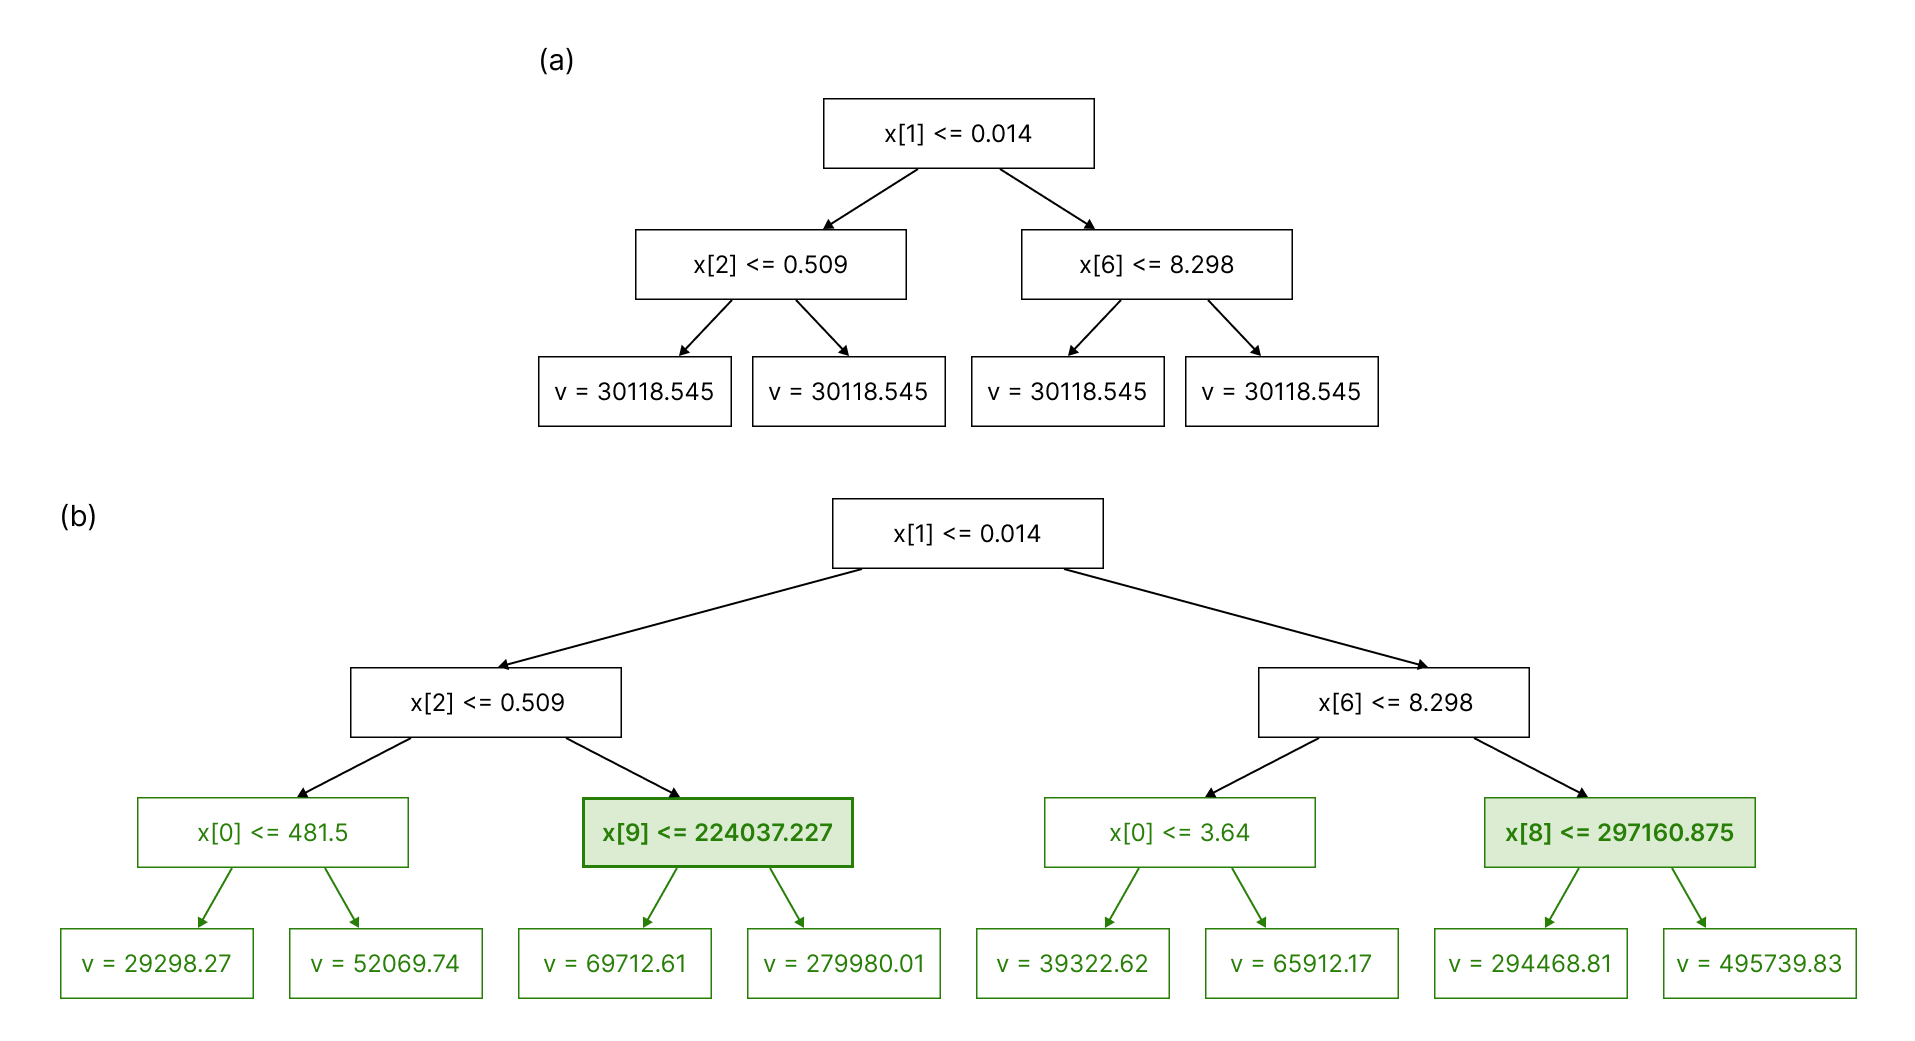
\includegraphics[width=1\textwidth]{figures/marco-metodologico/SK.png}
\caption{Árbol inicial (a) y extendido (b) entrenado sobre dataset House\_8L que tiene 8 features originales.}
\end{figure}
\label{figure3}

En cuanto a aspectos implementativos, esta alternativa fue la más desafiante. En un principio, la idea más natural era tomar toda la información de la estructura de los árboles iniciales para así, al crear los árboles extendidos, se fuerce el algoritmo a seguir la misma estructura que el árbol original hasta la profundidad  \texttt{initial\_max\_depth}. Sin embargo, eso conlleva el desafío de manejo memoria más minucioso. Es por ello que, luego de varias pruebas, surgió la idea que en el lugar de pasar la información original de los árboles, se construyan nuevos árboles con el algoritmo original pero limitando a que no se puedan utilizar las features provenientes del intercambio de información hasta alcanzar la \texttt{initial\_max\_depth}. Gracias a que tanto el entrenamiento original y extendido se realizan bajo la misma semilla, la correspondencia estre los mismos está garantizada.

Esta alternativa, no sólo es más eficiente en el uso de memoria, sino que también requiere menos modificaciones al algoritmo de construcción. En este caso tuvimos que implementar en Cython una nueva versión del \texttt{Splitter}, clase encargada de buscar los mejores cortes en cada paso de la construcción. La modificación centralmente limita las features disponibles hasta alcanzar el nivel dado por \texttt{initial\_max\_depth}, sacrificando ciertas optimizaciones del algoritmo con el fin de garantizar la correspondencia entre los árboles iniciales y sus extendidos.

En cuanto al método \texttt{predict} del modelo \texttt{SharedKnowledgeRandomForestRegressor}, es necesario notar ciertas particularidades. Para que nuevas muestras puedan atravesar los árboles de decisión extendidos, es necesario que cuenten con la misma cantidad de features que en entrenamiento. Es decir, así como durante entrenamiento cada árbol incorporó las predicciones de sus pares en su versión inicial, en predicción debe suceder lo mismo. Es así que para predecir nuevas observaciones, las mismas serán primero computadas por los árboles iniciales y esas predicciones se agregarán como features para ahora sí poder ser procesadas por los árboles extendidos.
Computadas las predicciones sobre cada árbol extendido, como en los restos de los modelos, se calcula la media dentro de cada grupo y luego se toma la media de los grupos para así conformar la predicción final del modelo.

\section{Optimización de hiperparámetros}

Una vez que los modelos con modificaciones al RF definidos, implementados y listos para ejecutarse, el siguiente paso es ajustar sus hiperparámetros para obtener la \textit{configuración óptima} que maximice su rendimiento.

Antes de avanzar con la optimización, es necesario separar los datasets seleccionados en conjuntos de entrenamiento y prueba (testing) para evaluar adecuadamente el modelo con datos “nunca antes vistos”, lo cual es esencial para validar hipótesis más adelante. En este caso, realizamos manualmente la división de los datos, asignando el $70\%$ al conjunto de entrenamiento y el $30\%$ al conjunto de testing. Luego, dividimos nuevamente el conjunto de entrenamiento en un $80\%$ para el entrenamiento propiamente dicho y un $20\%$ para validación. Esto permite evaluar las distintas configuraciones de hiperparámetros de manera adecuada, evitando el uso de los datos reservados para testing.

En cuanto a los hiperparámetros, además de los originales de Random Forest, como \texttt{n\_estimators}, \texttt{max\_depth} y \texttt{max\_features}, también tenemos que ajustar los nuevos hiperparametros que introducimos a nuestros modelos, como \texttt{group\_size}, \texttt{percentile} e \texttt{initial\_max\_depth}. 

Para encontrar los valores óptimos para estos hiperparámetros, inicialmente consideramos una búsqueda exhaustiva conocida como \textit{Grid Search}. Este método de búsqueda implica explorar todas las combinaciones posibles de los hiperparámetros definidos dentro de un rango preestablecido. Cada combinación se evalúa utilizando el error cuadrático medio (MSE) y así se puede encontrar la combinación “ganadora”, la de menor MSE. 

Debido a limitaciones de tiempo y recursos computacionales, no fue factible explorar todas las combinaciones posibles de hiperparámetros de manera exhaustiva. En cambio, decidimos realizar un muestreo aleatorio, con distribución uniforme, sobre una grilla predefinida, evaluando únicamente un subconjunto de combinaciones.

El procedimiento entonces conllevó los siguientes pasos: 

\begin{enumerate}
    \item Para cada modelo y cada dataset de los principales, se entrenó con los datos de entrenamiento y se buscaron las predicciones con el conjunto de validación para todas las configuraciones de hiperparámetros muestreadas en la grilla. Con las predicciones obtenidas calculamos su performance mediante el MSE.

    \item Luego, seleccionamos las 50 mejores configuraciones para cada dataset y modelo.
    
    \item Las combinaciones seleccionadas se unieron, obteniendo un total de 150 combinaciones por modelo (descartando los casos donde había combinaciones repetidas). Estas fueron re-evaluadas en los tres datasets, permitiendo probar en todos los datasets las mejores combinaciones encontradas en los distintos muestreos.
    
    \item Finalmente, luego de analizar los resultados obtenidos, definimos los hiperparámetros óptimos predeterminados para cada modelo.
\end{enumerate}

El proceso de definición de hiperparámetros predeterminados por modelo no fue una tarea sencilla. Para llevarlo a cabo, nos enfocamos en buscar identificar patrones entre los hiperparámetros a lo largo de los distintos conjuntos de entrenamiento. En particular, nos enfocamos en los dos parámetros centrales en nuestra hipótesis: \texttt{n\_estimators} y \texttt{group\_size}. Los mismos son importantes dado que controlan la cantidad de grupos y el tamaño de ellos. En las Figuras \hyperref[figure4]{4}, \hyperref[figure5]{5}, \hyperref[figure6]{6}, \hyperref[figure7]{7}, \hyperref[figure8]{8} y \hyperref[figure9]{9} se pueden observar mapas de calor que relacionan estas variables junto con el rendimiento de cada combinación evaluada mediante el MSE. Aquellas casillas en gris, indican combinaciones no factibles o no exploradas durante la exploración de la grilla.

\begin{figure}[h]
\centering
    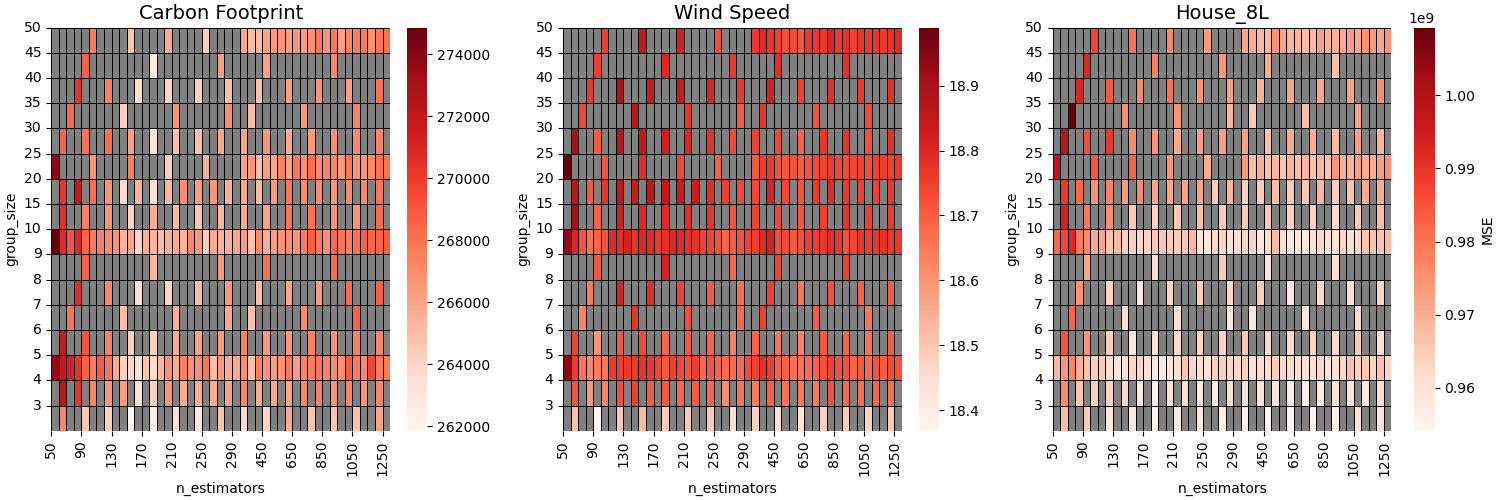
\includegraphics[width=1\textwidth]{figures/marco-metodologico/heatmaps/heatmap_iqr.png}
\caption{Relación entre hiperparámetros y MSE para el modelo \texttt{IQRRandomForestRegressor}}
\end{figure}
\label{figure4}

\begin{figure}[h]
\centering
    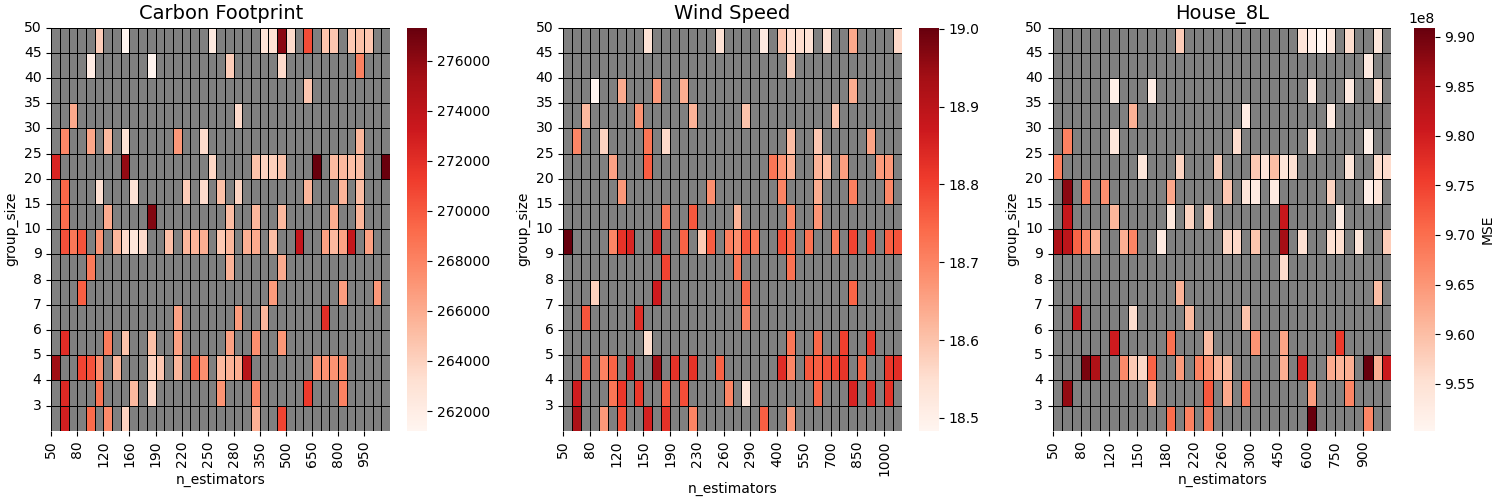
\includegraphics[width=1\textwidth]{figures/marco-metodologico/heatmaps/heatmap_pt_2.png}
\caption{Relación entre hiperparámetros \texttt{group\_size} y \texttt{n\_estimators} y MSE para el modelo \texttt{PercentileTrimmingRandomForestRegressor} con \texttt{percentile=2}}
\end{figure}
\label{figure5}

\begin{figure}[h]
\centering
    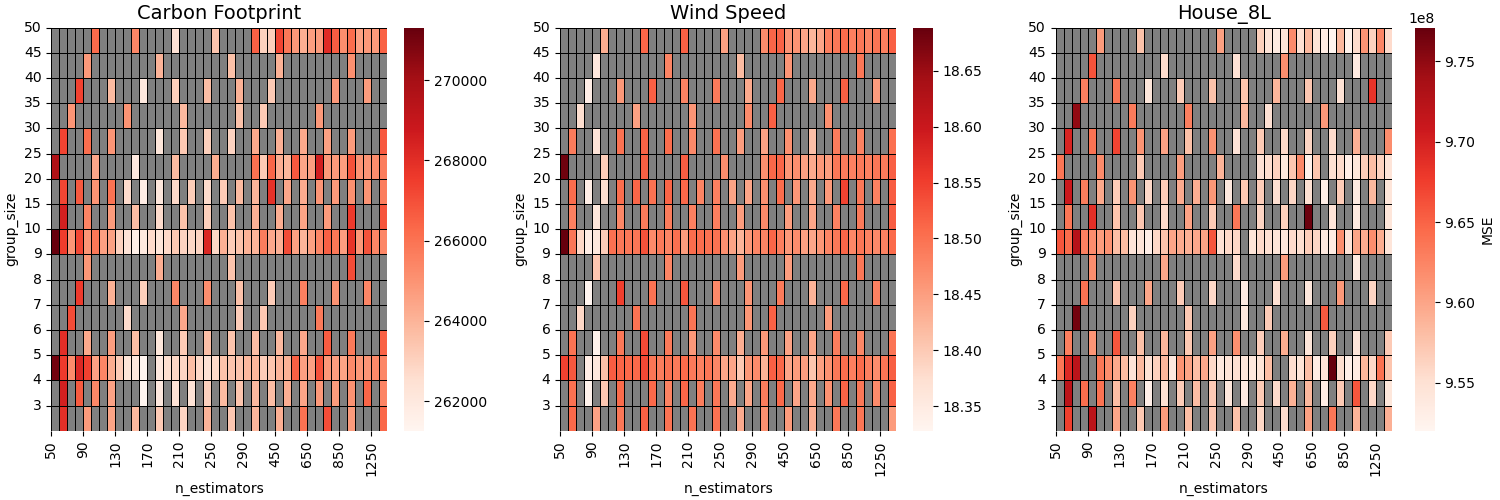
\includegraphics[width=1\textwidth]{figures/marco-metodologico/heatmaps/heatmap_oob.png}
\caption{Relación entre hiperparámetros \texttt{group\_size} y \texttt{n\_estimators} y MSE para el modelo \texttt{OOBRandomForestRegressor}}
\end{figure}
\label{figure6}

\begin{figure}[h]
\centering
    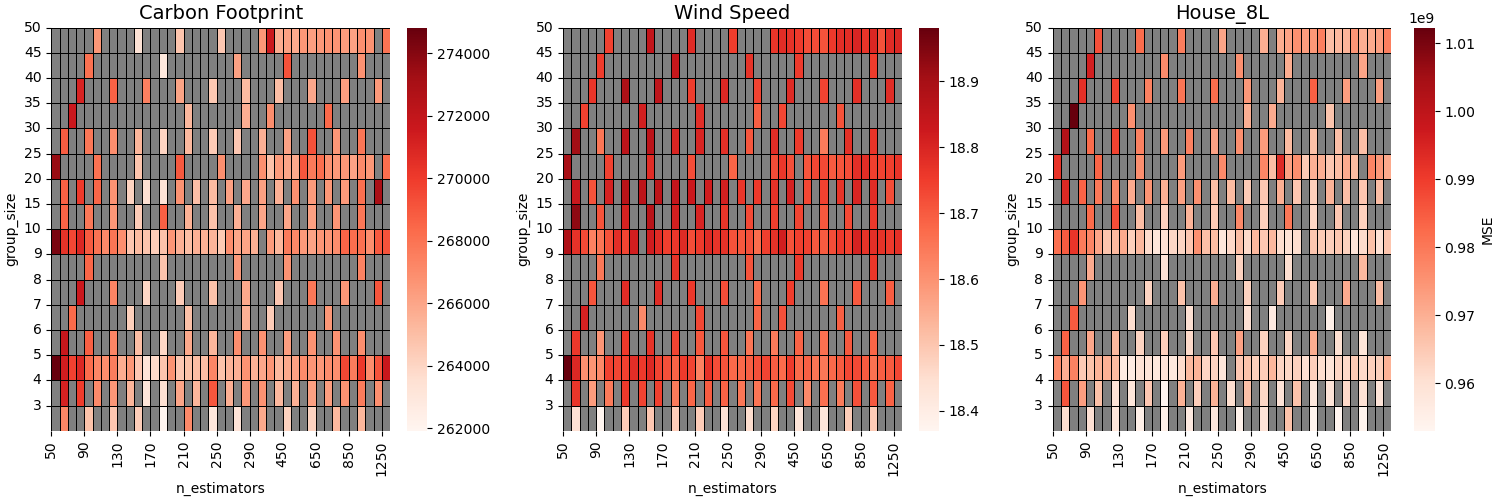
\includegraphics[width=1\textwidth]{figures/marco-metodologico/heatmaps/heatmap_oob_plus_iqr.png}
\caption{Relación entre hiperparámetros \texttt{group\_size} y \texttt{n\_estimators} y MSE para el modelo \texttt{OOBPlusIQRRandomForestRegressor}}
\end{figure}
\label{figure7}

\begin{figure}[h]
\centering
    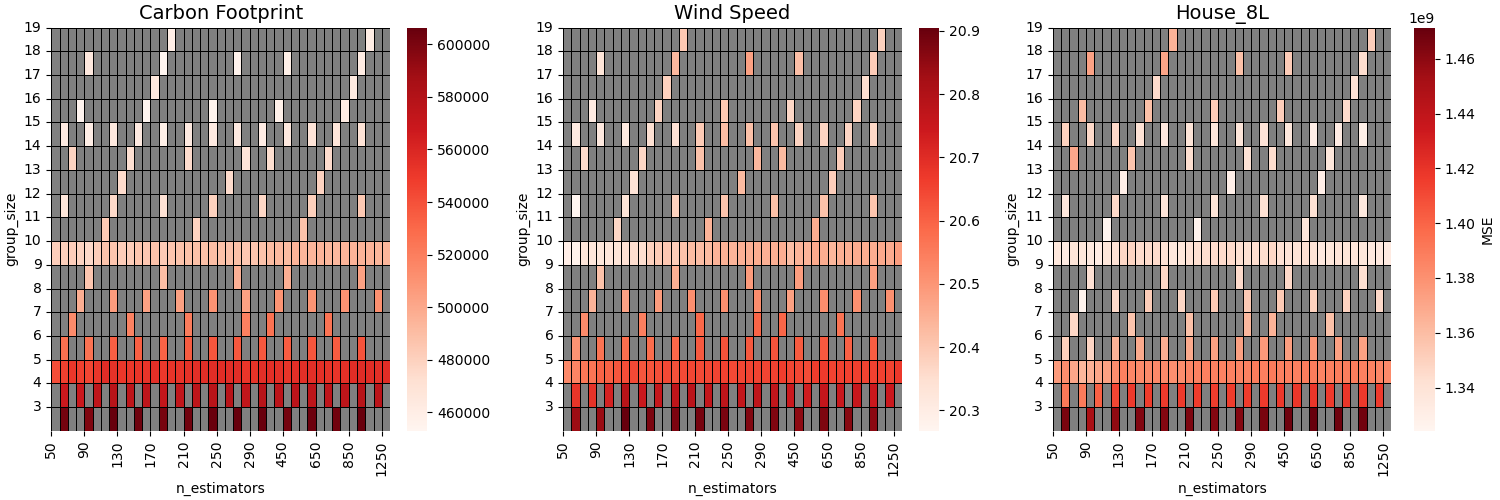
\includegraphics[width=1\textwidth]{figures/marco-metodologico/heatmaps/heatmap_fsc.png}
\caption{Relación entre hiperparámetros \texttt{group\_size} y \texttt{n\_estimators} y MSE para el modelo \texttt{FirstSplitCombinerRandomForestRegressor}}
\end{figure}
\label{figure8}

\begin{figure}[h]
\centering
    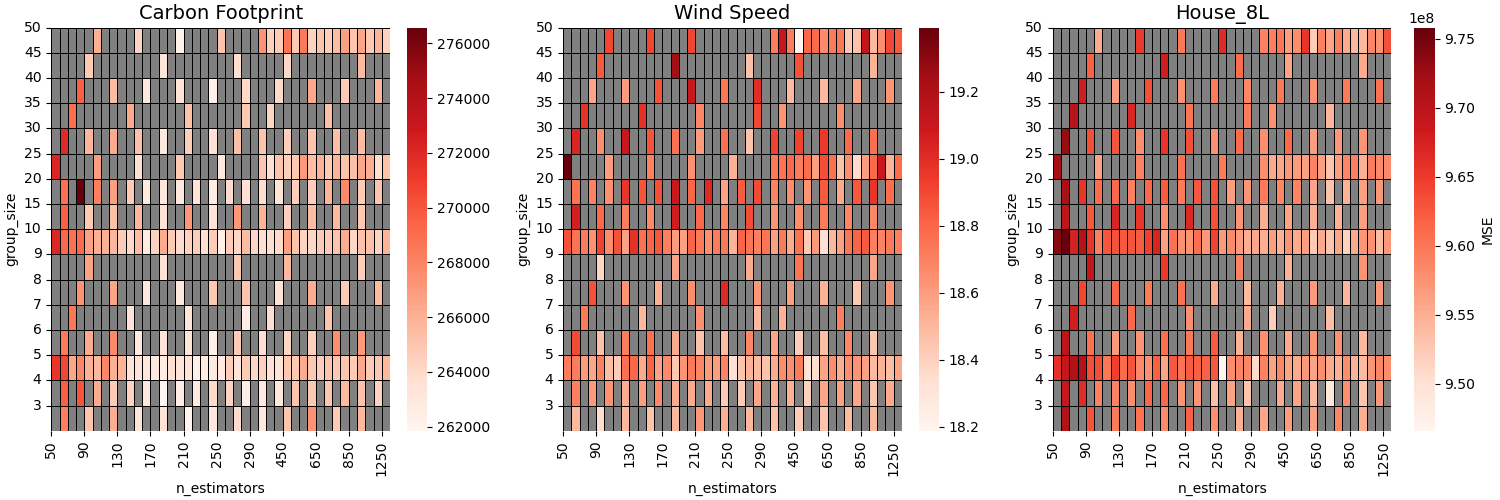
\includegraphics[width=1\textwidth]{figures/marco-metodologico/heatmaps/heatmap_sk.png}
\caption{Relación entre hiperparámetros \texttt{group\_size} y \texttt{n\_estimators} y MSE para el modelo \texttt{SharedKnowledgeRandomForestRegressor}}
\end{figure}
\label{figure9}

\FloatBarrier

\begin{figure}[h]
\centering
    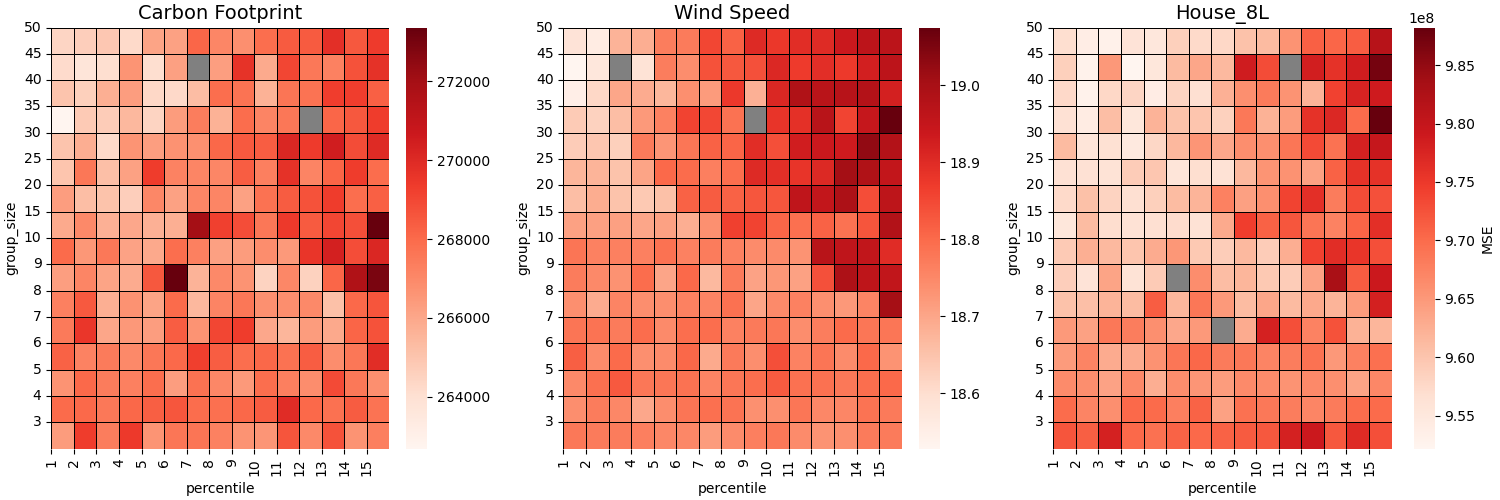
\includegraphics[width=1\textwidth]{figures/marco-metodologico/heatmaps/heatmap_percentile_vs_group_size.png}
\caption{Relación entre hiperparámetros \texttt{group\_size} y \texttt{percentile} y MSE para el modelo \texttt{PercentileTrimmingRandomForestRegressor}}
\end{figure}
\label{figure10}



Un patrón en común entre todos los modelos y los datasets es que, en general, las configuraciones de hiperparámetros que mejor resultados obtienen son aquellas que tienen un número moderado de árboles total (entre $100$ y $300$) y grupos de tamaños relativamente chicos. Esto de puede notar en los mapas de calor observando el tono más claro de las esquinas inferiores izquierdas. Sin embargo, hay dos modelos los cuáles tienen particularidades.

Para el caso particular del \texttt{FirstSplitCombinerRandomForestRegressor}, se nota claramente con los mapas de calor que este modelo requiere tamaños de grupos mayores, dado que la parte inferior de los mismos se los ve más oscuros indicando mayor MSE, es decir peor rendimiento. Esto tiene muchos sentido dado la naturaleza misma del modelo. Al depender la capacidad predictiva del modelo en los árboles combinados por grupo y considerando que se toma el primer corte de cada árbol del grupo, cuanto mayor sea el tamaño del grupo mayor será la profundidad de los árboles combinados, permitiendo capturar más información de los datos.

Por su parte, en cuanto al modelo \texttt{PercentileTrimmingRandomForestRegressor}, en la \hyperref[figure10]{Figura 10} se observa la relación entre los hiperparámetros \texttt{group\_size} y \texttt{percentile}, donde se puede observar que las mejores combinaciones entre estos dos ocurre con un tamaño de grupo grande y porcentaje de exclusión en los extremos bajos. Esto tiene sentido dado que, a diferencia del modelo que utiliza IQR, este siempre elimina de ambos extremos por lo que para no perder tanta información en el promedio grupal, se necesitan más árboles por grupo. A su vez, percentiles mayores a 5 ya significa la pérdida de mucha información. Por esto motivo se ve que la \hyperref[figure5]{Figura 5} se filtran aquellas configuraciones dónde se uso percentil igual a dos, para a partir de ahí notar la cantidad de árboles totales más óptima.

Para los demás hiperparámetros específicos de cada modelo como \texttt{initial\_max\_depth} o \texttt{max\_features}, se definieron una vez establecidos los principales a partir de la  comparación simple del valor de MSE de las distintas configuraciones. El hiperparámetro \texttt{max\_features} fue sólo tenido en cuenta en \texttt{FirstSplitCombinerRandomForestRegressor} dado que era dónde se veía más neceserario ajustarlo. Para el resto de modelos se dejó este hiperparámetro como se ecuentra en el default de la librería de código abierto, que es en $1$, es decir que se usan todas las features en todos los árboles. 

El caso del hiperparámetro \texttt{max\_depth} fue un caso particular. Al ser un parámetro de naturaleza regularizador ya que controla que los árboles no sobre-ajusten a los datos, el mismo depende mucho del problema a evaluar, es decir del dataset. Por eso motivo, se decidió no definir un valor predeterminado para el mismo, sino que esté optimizado según cada modelo y dataset.

En base al análisis global de los hiperparámetros y su interrelación fue que quedaron conformados los valores predeterminados para cada modelo y dataset. Si bien el procedimiento llevado a cabo no asegura encontrar la configuración óptima \textit{global}, permite identificar parámetros con un desempeño eficiente dentro de un tiempo razonable.

\section{Comparación de modelos}

Teniendo los modelos con sus hiperparámetros definidos\footnote{Valores por modelo y dataset en \hyperref[appendix7]{Apéndice 7}.}, utilizamos los datos reservados para testing para evaluar si alguno presenta mejoras significativas en desempeño en comparación con el algoritmo original \textbf{\texttt{RandomForestRegressor}}. Para esto debemos llevar a cabo un test no paramétrico llamado Kruskal-Wallis, el cual se basa en las siguientes hipótesis:

\begin{itemize}
    \item \textit{Hipótesis nula ($H_0$)}: No hay diferencias significativas en el MSE entre los modelos evaluados, incluido el \texttt{RandomForestRegressor}.

    \item \textit{Hipótesis alternativa ($H_1$)}: Al menos uno de los modelos tiene un MSE significativamente diferente al de \texttt{RandomForestRegressor}.
\end{itemize}

El siguiente procedimiento se llevó a cabo para los tres datasets principales, y luego los otros tres adicionales. En primer lugar, realizamos una validación cruzada de 10-folds, asegurándonos de que todos los modelos utilicen exactamente los mismos conjuntos de entrenamiento y validación mediante una semilla. Esto genera, para cada modelo, un conjunto de 10 valores de MSE, y se agrupan en una lista específica para cada modelo. 

Con las listas generadas, usamos el test de \textit{\textbf{Kruskal-Wallis}} (KW) para comparar simultáneamente los MSEs de todos los modelos. Este análisis permite identificar si existen diferencias significativas entre los modelos; un valor alto en el test KW, y su p-valor asociado, indica dichas diferencias. 

El test Kruskal-Wallis permite identificar si existen diferencias significativas entre los modelos evaluados, pero no proporciona información sobre cuáles modelos específicos presentan dichas diferencias. Debido a esto, en caso en que se rechace la hipótesis nula ($H_0$) y obtenemos un p-valor menor a $0.05$, realizamos un análisis \textit{post-hoc} utilizando el test de \textit{Dunn} para determinar qué pares de modelos son significativamente diferentes. De este test se obtendrá una matriz, presentada en \hyperref[ch::capitulo7]{\textit{Resultados}}, que compara cada modelo con los demás para identificar dónde están las diferencias.
